\documentclass[12p,a4paper]{article}
\usepackage{amsmath}
\usepackage{graphicx}
\usepackage{hyperref}
\pagenumbering{gobble}
\graphicspath{ {images/} }
\title{Short \& Simple Guide to Robotics Development}
\author{Alex Balgavy}

\begin{document}
\maketitle
\newpage
\tableofcontents
\newpage

\section{General Information}
\subsection{Methods}
\paragraph{init()}
The init method is what runs when you press the initialize button on the phone. Usually used to set up variables and prepare the robot for start.

\paragraph{loop()}
This method runs when the play button is pressed on the phone. It repeats (loops) over and over during the TeleOp method. This means that it always runs. It contains all of the statements to move motors and servos.

\subsection{The Register}
The file \verb!FtcOpModeRegister.java! is the file that decides which op modes are sent to the phone. Here is an example of a line in the file:

\begin{verbatim}
manager.register("TeleOp", TeleOp.class);
\end{verbatim}

In this statement, \verb!manager.register()! is the method that registers the op mode, taking two arguments --- the name displayed on the phone (``TeleOp'') and the java file (\verb!TeleOp.class!).\\
In order for your op mode to upload to the phone, you \textbf{need} to add a new line to this file with the program. Otherwise, your program \textbf{will not upload}.

\section{Writing an opmode}
\subsection{Wiring}

Before you start programming, you need to make sure that the robot is correctly wired. Here's an example of how the robot should be wired:\\
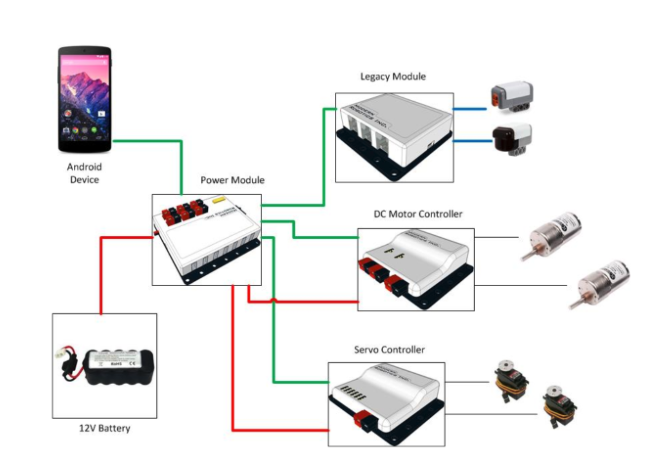
\includegraphics[scale=0.3]{robot-wiring}\\
You need to make sure that the cables are connected everywhere.

\subsection{Robot Configuration}

On the phone, you need to check the profile every time you change the wiring. Click the three dots in the top right corner, click settings, and configure robot. Click the `edit' button under the title `'Robot'' and click the legacy module. Edit each of the controllers and check to see if the ports match the hardware.
\subsection{Programming}

\paragraph{Defining variables}Before anything starts running, you need to define your variable types. Motors are of class DcMotor, servos are of class Servo. Here's what our definitions look like in our code:

\begin{verbatim}
DcMotor motorRight;
DcMotor motorLeft;
DcMotor motorTurboRight;
DcMotor motorTurboLeft;
Servo middleRelease;
\end{verbatim}

You can also set up any other variables.

\paragraph{Mapping hardware to software}In the \verb!init()! method, you get the hardware and save it to variables in the software. Like so:

\begin{verbatim}
// Main motor
motorLeft = hardwareMap.dcMotor.get("rMain");

// Servo
middleRelease = hardwareMap.servo.get("release");
\end{verbatim}

The variables in the \verb!get()! method \textbf{have to match} the variables that you set up in the phone profile.

\paragraph{Getting values from joysticks and writing them to motors} Get the values from joysticks:

\begin{verbatim}
float right = gamepad1.right_stick_y;
float left = gamepad1.left_stick_y;
\end{verbatim}

Clip and scale the input:

\begin{verbatim}
right = Range.clip(right, -1, 1);
left = Range.clip(left, (float) -1.0, (float) 1.0);
        
right = (float) scaleInput(right);
left = (float) scaleInput(left);
\end{verbatim}

Finally, write values to the motors:

\begin{verbatim}
motorRight.setPower(right);
motorLeft.setPower(left);
\end{verbatim}

\paragraph{Moving servos} Write an if statement with a true/false condition (button is down or not), and based on that it moves the servo. Use a variable that takes care of tracking the servo position. Servos can have position between 1.0 and 0.0 inclusive, so check if changing the variable would break the bounds, and if it would, set it to the max/min. Here's what the code is:

\begin{verbatim}
if (gamepad1.a) {
	if (releasePosition + 0.1 > 1.0) {
		releasePosition = 1.0;
	} 
	else {
		releasePosition += 0.1;
	}
	middleRelease.setPosition(releasePosition);
} 
else if (gamepad1.x) {
	if (releasePosition - 0.1 < 0.0) {
		releasePosition = 0.0;
	} 
	else {
		releasePosition -= 0.1;
	}
	middleRelease.setPosition(releasePosition);
}
\end{verbatim}

\paragraph{Comments} Make sure that you comment everything you do, it will be easier for other programmers to understand. You can use \verb!//region NAME! and \verb!//endregion! for collapsible comments.

\section{Git \& Github}
\subsection{Git basics}

\paragraph{What is Git \& Terms} Git is a VCS (version control system). It tracks all the changes you make to files and creates `snapshots' of those versions. You can go back to any version any time you want. The snapshots are called `commits'. When you `commit', you create a snapshot. When you `push', you upload it to a remote repository (a server that stores the code, such as Github). When you `pull', you get changes to any files that are not synced to your local version of the files. \href{https://desktop.github.com}{Github Desktop} does all of this for you with a button called `sync'. 

\paragraph{Committing} When you make a commit, you have to write in a message. You select which files you want to commit, type in a message, and click the commit button. Then you click sync to upload your changes.

\paragraph{Reverting a commit} Select a specific commit in the timeline, click the cog wheel in the view on the right, and click revert commit.

\subsection{Branches}

A branch is a `copy' of a snapshot. Let's say you're working on the `master' branch (the original code), and you want to make a larger change without breaking anything. You would create a branch, and work on that branch, without changing anything in the original code. Once your changes are complete and functional, you would merge that branch back into the `master' branch.\\
Here's a diagram of how branches work in the project history:\\
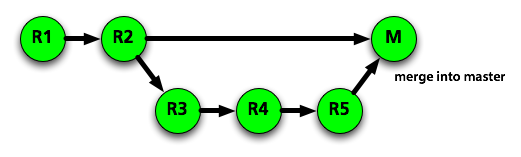
\includegraphics[scale=0.6]{git-branches}\\ \\
This is where you manage branches in Github Desktop:\\\\
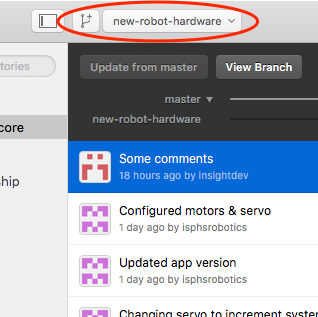
\includegraphics[scale=0.6]{github-desktop-branches}

\subsection{Github}

\paragraph{Downloading code}Github is used to share code. Our Github repository URL is \url{http://github.com/isphsrobotics/robot-core}. To download the code, go to this repo, and click the icon next to `'Download ZIP'':\\
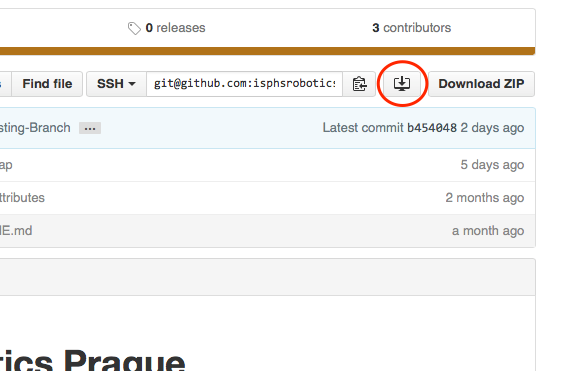
\includegraphics[scale=0.6]{download-repo}
\paragraph{Implementing your changes}To implement changes, you create a pull request. When you're on your branch, sync it, and then click the button in the top right corner labelled `Pull Request'.

\subsection{Standard Git Workflow}
\textbf{Please do this for any large changes you want to implement:}

\begin{enumerate}
\item{Sync newest code from Github (use the `sync' button).}
\item{Create a new branch and check it out (git language for `switch to it').}
\item{Make your changes on that branch, including any commits.}
\item{Submit a pull request, using the `pull request' button on the top right.}
\item{Wait to see if you pull request gets approved.}
\end{enumerate}

\textbf{DO NOT MAKE ANY LARGE CHANGES ON THE MASTER BRANCH.} That way, we can check any changes for potential problems.

\section{Further information}

Here are some useful links if you want to learn more about any of these concepts:

\begin{itemize}
\item{\href{https://github.com/ftctechnh/ftc_app}{The FTC repository}}
\item{\href{https://github.com/ftctechnh/ftc_app/blob/master/doc/tutorial/FTCTraining_Manual.pdf}{The official FTC training manual}}
\item{\href{https://try.github.io/}{Git -- interactive command-line tutorial (15 minutes)}}
\item{\href{https://guides.github.com}{Github guides}}
\end{itemize}
\end{document}